\section{Method}
\label{section:method}

%   - Introduction
In this section we describe the combined isochrone fitting and gyrochronology
model implemented in \sd.
% A common approach to stellar age-dating is to make separate age predictions
% using separate sets of observables.
% For example, if a star's rotation period, parallax, and apparent magnitudes in
% a range of bandpasses are available, it is possible to predict its age from
% both gyrochronology and isochrone fitting separately.
% How these two age predictions are later combined is then a difficult choice.
% Is it best to average these predictions, to use the more precise of the two,
% or the one believed to be more accurate?
% The methodology described here provides an objective method for combining age
% estimates.
% There is, after all, only one age for each star.
Combining information from different models can be relatively simple, as long
as the processes being modeled; those that generated the data, are
independent.
In this case, we are combining information that relates to the burning of
hydrogen in the core, which translates to CMD or HRD position,
% (this is the process that drives the slow increase in \teff\ and luminosity
% over time)
with information about the magnetic braking history of a star (the current
rotation period).
We can assume that, to first order, these two processes are independent: the
hydrogen fraction in the core does not affect a star's rotation period and
vice versa.
These processes are not truly independent, however any dependence here is
unlikely to affect our results within the uncertainties.
If this assumption is valid, the likelihoods calculated using each model can
be multiplied together.

The desired end product of this method is an estimate of the non-normalized
posterior probability density function (PDF) over the age of a star,
\begin{equation} \label{eqn:eqn1}
    p(A|{\bf m_x}, T_{\mathrm{eff}}, \log(g), \hat{F},
    P_{\mathrm{rot}}, \bar{\omega}),
\end{equation}
where $A$ is age, ${\bf m_x}$ is a vector of
apparent magnitudes in various bandpasses, \fhat\ is the {\it observed} bulk
metallicity, \prot\ is the rotation period and \pmega\ is parallax.
In order to calculate a posterior PDF over age, we must marginalize over
parameters that relate to age, but are not of interest in this study.
These parameters include equivalent evolutionary point (which we abbreviate to
EEP or $E$), which is a dimensionless number ranging from around 200 for M
dwarfs up to around 500 for subgiants and is 355 for the Sun
\citep[see][]{dotter2016, choi2016}.
Stars are defined as subgiants when their EEP exceeds 454.
Mass is uniquely defined by EEP, age and metallicity.
The other parameters are distance ($D$), V-band extinction ($A_V$) and the
{\it inferred} bulk metallicity, $F$.
The marginalization involves integrating over these extra parameters,
\begin{eqnarray} \label{eqn:bayes}
    & p(A|{\bf m_x}, T_{\mathrm{eff}}, \log(g), \hat{F},
    P_{\mathrm{rot}}, \bar{\omega})
\\ \nonumber
    & \propto \int p({\bf m_x}, T_{\mathrm{eff}}, \log(g), \hat{F},
    P_\mathrm{rot}, \bar{\omega}|
    A, E, D, A_V, F)~p(A)p(E)p(D)p(A_V)p(F)dEdDdA_VdF.
\end{eqnarray}
This equation is a form of Bayes' rule,
\begin{equation} \label{eqn:eqn2}
\mathrm{Posterior} \propto \mathrm{Likelihood} \times \mathrm{Prior},
\end{equation}
where the likelihood of the data given the model is,
\begin{equation} \label{eqn:full_likelihood}
    p({\bf m_x}, T_{\mathrm{eff}}, \log(g), \hat{F}, \bar{\omega},
    P_{\mathrm{rot}}|A, E, D, A_V, F),
\end{equation}
and the prior PDF over parameters is,
\begin{equation} \label{eqn:prior}
    p(A)p(E)p(D)p(A_V)p(F).
\end{equation}

%   - Why iso and gyro are independent.
Not all of the observables on the left of the `$|$' in the likelihood depend
on all of the parameters to the right of it.
For example, rotation period, \prot\ does not depend on V-band extinction,
$A_V$.
In our model, we make use of conditional independencies like this and use them
to factorize the likelihood.
Instead of the likelihood of equation \ref{eqn:full_likelihood},
where every observable depends on every parameter, our model can be factorized
as,
\begin{equation} \label{eqn:factorized}
    p({\bf m_x}, T_{\mathrm{eff}}, \log(g), \hat{F}, \bar{\omega}
    |D, A_V, F, A, E, M, C_{B-V}) ~p(P_\mathrm{rot}|A, E, M, C_{B-V}),
\end{equation}
where we have introduced two new parameters, $C_{B-V}$, which is the $B-V$
color that is often used as a mass proxy in the literature and mass itself
($M$), which is used in our gyrochronology model to calculate convective
turnover time and therefore Rossby number.
The above factorization of the likelihood describes the fact that, in our
model, rotation period does not depend directly on distance, extinction or
metallicity.
EEP, age, metallicity, extinction and distance determine the observed
spectroscopic properties (\teff, \logg, \feh) and apparant magnitudes, ${\bf
m_x}$) as well as the \cbv\ color and mass of a star.
In turn, it is a star's age, \cbv\ color, mass and EEP that determine its
rotation period.
Breaking up the problem this way allows us to easily combine isochronology and
gyrochronology and infer the joint age of a star from all its observables.
While true that rotation period also depends on metallicity at some level, we
assume that this dependency is weak enough not to significantly affect the
ages that we infer.

% $C_{B-V}$ and $M$ are not measured but {\it inferred}: they are latent
% parameters.
% We infer $C_{B-V}$ because many stars do not have a directly measured $B-V$
% color.
% For example, most \kepler\ stars have {\it 2MASS} photometry in J, H and K
% bands and \Gaia\ photometry in $G$, $G_{BP}$ and $G_{RP}$, but do not all have
% B and V band colors.
% However, the gyrochronology model we use is calibrated to B-V color, not J-K
% or otherwise \citep{barnes2007, mamajek2008, angus2015}.
% % A probabilistic graphical model (PGM) depicting the joint probability over
% % parameters and observables is shown in figure \ref{fig:PGM}.
% % It describes the conditional dependencies between parameters (in white
% % circles) and observables (in grey circles) with arrows leading from the causal
% % processes to the dependent processes.
% For example, it is the mass, age, metallicity, extinction and distance that
% determines the observed spectroscopic properties (\teff, \logg, \feh)
% and apparant magnitudes, ${\bf m_x}$).
% These parameters also determine the \cbv\ color of a star.
% In turn, it is a star's age and \cbv\ color that determine its rotation
% period.
% Note that, written this way, stellar rotation periods do not directly depend
% on stellar mass.
% Mass, age and metallicity determine $C_{B-V}$, and $C_{B-V}$ along with age
% determines rotation period.
% The purpose of this PGM is not to depict the physical realities of stellar
% evolution, it is only a visual description of the structure of the model we
% use here.
% Breaking up the problem this way allows us to efficiently join isochronology
% and gyrochronology and infer the joint age of a star from all its observables.
% It may well be that rotation period depends directly on mass and metallicity
% in reality, but it is more practical for us to assume that these dependencies
% are weak enough not to significantly affect the ages that we ultimately infer.

%   - The formulas
The factorization of the likelihood described in equation \ref{eqn:factorized}
allows us to multiply two separate likelihood functions together: one computed
using an isochronal model and one computed using a gyrochronal model.
We assume that the probability of observing the measured observables, given
the model parameters is a Gaussian and that the observables are identically
and independently distributed, so we use Gaussian likelihood functions.
The isochronal likelihood function is,
\begin{eqnarray} \label{eqn:isochrones_only_likelihood}
    & \mathcal{L_{\mathrm{iso}}} = p({\bf m_x}, T_{\mathrm{eff}}, \log(g),
    \hat{F},
    \bar{\omega}, C_{B-V}|A, E, D,
    A_V, F) \\ \nonumber
    & = \frac{1}{\sqrt{(2\pi)^n \det(\Sigma)}}
    \exp\left( -\frac{1}{2} ({\bf O_I} - {\bf I})^T \Sigma ^{-1}
    ({\bf O_I} - {\bf I})\right),
\end{eqnarray}
where ${\bf O_I}$ is the n-dimensional vector of $n$ observables: \teff,
\logg, \fhat, \pmega, ${\bf m_x}$ (where $n$ is 4 plus the number of
apparant magnitudes in different pass-bands that are available) and $\Sigma$
is the covariance matrix of that set of observables.
${\bf I}$ is the vector of {\it model} observables that correspond to a set of
parameters: $A$, EEP, $F$, $D$ and $A_V$, calculated using an isochrone model.
We assume there is no covariance between these observables and so this
covariance matrix consists of individual parameter variances, added in
quadrature to an additional variance that depends on B-V color and
evolutionary stage, along the diagonal with zeros everywhere else.
The additional variance is described in more detail later in this section.
The gyrochronal likelihood function is,
\begin{eqnarray} \label{eqn:gyro_likelihood}
    & \mathcal{L_{\mathrm{gyro}}} = p(P_\mathrm{rot} |A, C_{B-V}, M) \\ \nonumber
    & = \frac{1}{\sqrt{(2\pi) \det(\Sigma_P)}}
    \exp\left( -\frac{1}{2} ({\bf P_O} - {\bf P_P})^T \Sigma ^{-1}
    ({\bf P_O} - {\bf P_P})\right),
    % = \prod_i \frac{1}{\sqrt{2\pi}\sigma_i} \exp
    % \left(-\frac{(P_{\mathrm{obs}, i} - P_{\mathrm{pred},
    % i})^2}{2\sigma_i^2}\right),
\end{eqnarray}
% where $P_{\mathrm{obs}, i}$ is the $i$th observed rotation period,
% $P_{\mathrm{pred}, i}$ is the corresponding predicted rotation period,
% calculated from the $i$th age and $C_{B-V}$ values predicted by the isochronal
% model.
where ${\bf P_O}$ is a 1-D vector of observed log-rotation periods, ${\bf
P_P}$ is the vector of corresponding predicted log-rotation periods,
calculated using the vector of ages and $C_{B-V}$ values that correspond to
the input parameters as predicted by the isochronal model.
The full likelihood function used in our model is the product of these two
likelihood functions,
\begin{eqnarray} \label{eqn:full_likelihood}
    & \mathcal{L_{\mathrm{full}}} = \frac{1}{\sqrt{(2\pi)^n \det(\Sigma)}}
    \exp\left( -\frac{1}{2} [{\bf O_I} - {\bf I}]^T \Sigma ^{-1}
    [{\bf O_I} - {\bf I}]\right) \\ \nonumber
    & \times
    \frac{1}{\sqrt{(2\pi) \det(\Sigma_P)}}
    \exp\left( -\frac{1}{2} [{\bf P_O} - {\bf P_P}]^T \Sigma ^{-1}
    [{\bf P_O} - {\bf P_P}]\right).
\end{eqnarray}

%   - Priors
We placed priors over the model parameters $A$, EEP, $F$, $D$ and $A_V$.
These distributions, described in the appendix, represent our prior beliefs
about the values these parameters will take, before using the data to update
those beliefs via a likelihood and produce a posterior belief about their
values.

% Practicalities: sampling, etc.
%-----------------------------------------------------------------------------
%- isochrones.py
To calculate ${\bf I}$, the vector of predicted isochronal observables, we
used the {\tt isochrones.py} {\it python} package which has a range of
functionalities relating to isochrone fitting.
The first of the {\tt isochrones.py} functions we used is the likelihood
function of equation \ref{eqn:isochrones_only_likelihood}.
The {\tt isochrones.py} likelihood function accepts a dictionary of
observables which can, but does not {\it have} to include, all of the
following: \teff, \logg, $F$, parallax and apparent magnitudes in a range of
colors, as well as the uncertainties on all these observables.
It then calculates the residual vector $({\bf O_I} - {\bf I})$ where ${\bf
O_I}$ is the vector of observables and ${\bf I}$ is a vector of corresponding
predicted observables.
The prediction is calculated using a set of isochrones \citep[we used the MIST
models,][]{paxton2011, paxton2013, paxton2015, dotter2016, choi2016,
paxton2018}, where the set of {\it model} observables that correspond to a set
of physical parameters is returned.
This requires interpolation over the model grids since, especially at high
dimensions, it is unlikely that any set of physical parameters will exactly
match a precomputed set of isochrones.
The observables that correspond to a set of physical parameters go into ${\bf
I}$ and the {\tt isochrones.py} likelihood function returns the result of
equation \ref{eqn:isochrones_only_likelihood}.
The second {\tt isochrones.py} function we used is one that predicts \cbv\ for
a given set of stellar parameters, which was then used to calculate the
gyrochronal likelihood function of equation \ref{eqn:gyro_likelihood}.

%   - Step-by-step description
The inference processes procedes as follows (as a reminder, we use {\it
observables} to refer to the data: \teff, \logg, etc and {\it parameters} to
refer to the model parameters: EEP, age, metallicity, distance and extinction.
First, a set of parameters: age, EEP, metallicity, distance and extinction, as
well as observables \teff, \logg, bulk metallicity, apparent magnitudes and
parallax (${\bf O_I}$) for a single star are passed to the isochronal
likelihood function, equation \eqref{eqn:isochrones_only_likelihood}.
Then, a set of {\it model} values of \teff, \logg, bulk metallicity, apparent
magnitudes and parallax (${\bf I}$) that correspond to that set of parameters
are calculated by {\tt isochrones.py}.
The isochronal log-likelihood, $\ln(\mathcal{L}_{\mathrm{iso}})$, is then
computed for these parameter values.
The same age that was passed to the likelihood function, and the $C_{B-V}$ and
mass corresponding to it, along with the observed rotation period, are then
passed to the gyrochronal likelhood function (equation
\ref{eqn:gyro_likelihood}).
The gyrochronal log-likelihood, $\ln(\mathcal{L}_{\mathrm{gyro}})$, is
computed.
The full log-likelihood is then calculated,
\begin{equation} \label{eqn:both_likelihood}
\ln(\mathcal{L}_{\mathrm{full}})
= \ln(\mathcal{L}_{\mathrm{iso}}) + \ln(\mathcal{L}_{\mathrm{gyro}}),
\end{equation}
and added to the log-prior to produce a single sample from the posterior PDF.

%   - The gyrochronology models
The gyrochronology model used to predict $\bf{P_P}$ was,
\begin{equation}
    P_\mathrm{rot} =\begin{cases}
        A^\eta \alpha (C_{B-V} - \delta)^\beta, & \text{if $Ro < 2$}. \\
        P_{\mathrm{max}}, & \text{if $Ro \geq 2$}.
    \end{cases}
\label{eqn:gyro}
\end{equation}
where \prot\ is rotation period in days, \cbv\ is a star's $B-V$ color, $A$ is
stellar age in Myrs and $\eta$, $\alpha$, $\beta$ and $\delta$ take values
0.55, 0.4, 0.31 and 0.45 respectively \citep{angus2015}.
This functional form was introduced by \citep{barnes2007} and the parameter
values are adopted from the recalibration performed in \citet{angus2015},
which is based on young cluster stars and old asteroseismic stars.
We adapted this classical gyrochronology model to incorporate the new
observations showing that magnetic braking ceases at a critical Rossby number
\citep{vansaders2016}.
The Rossby number, $Ro$, is the ratio of rotation period to convective
overturn time $P_{\mathrm{rot}}/\tau$ and determines whether a star is still
undergoing magnetic braking ($Ro < 2$) or has stopped spinning down and
retains its terminal rotation period, $P_\mathrm{max}$, which is the period it
had as it reached the critical Rossby number of 2 \citep{vansaders2016}.
The convective overturn time, $\tau$, was estimated using equation 11 of
\citet{wright2011}.
Figure \ref{fig:rotation_model} shows the rotation periods of 841
simulated stars with rotation periods generated from the gyrochronology model.
\begin{figure}
  \caption{
The rotation period model.
Late F, GK and early M dwarfs follow the \citet{angus2015} gyrochronology
relation, with the exception of old, slowly rotating stars with large Rossby
numbers whose rotation periods are fixed at 2$\times$ their convective
overturn time.
The rotation periods of early F, late M dwarfs and subgiants were generate
    from a log-normal distribution with standard deviation shown in figure
    \ref{fig:variance}.
The top panel shows the rotation periods vs. B-V colors of simulated stars,
    colored by their age and the bottom panel shows the same stars colored
    by their equivalent evolutionary point (EEP).
    The gray lines describe the \citep{angus2015} gyrochronology model.
}
  \centering
    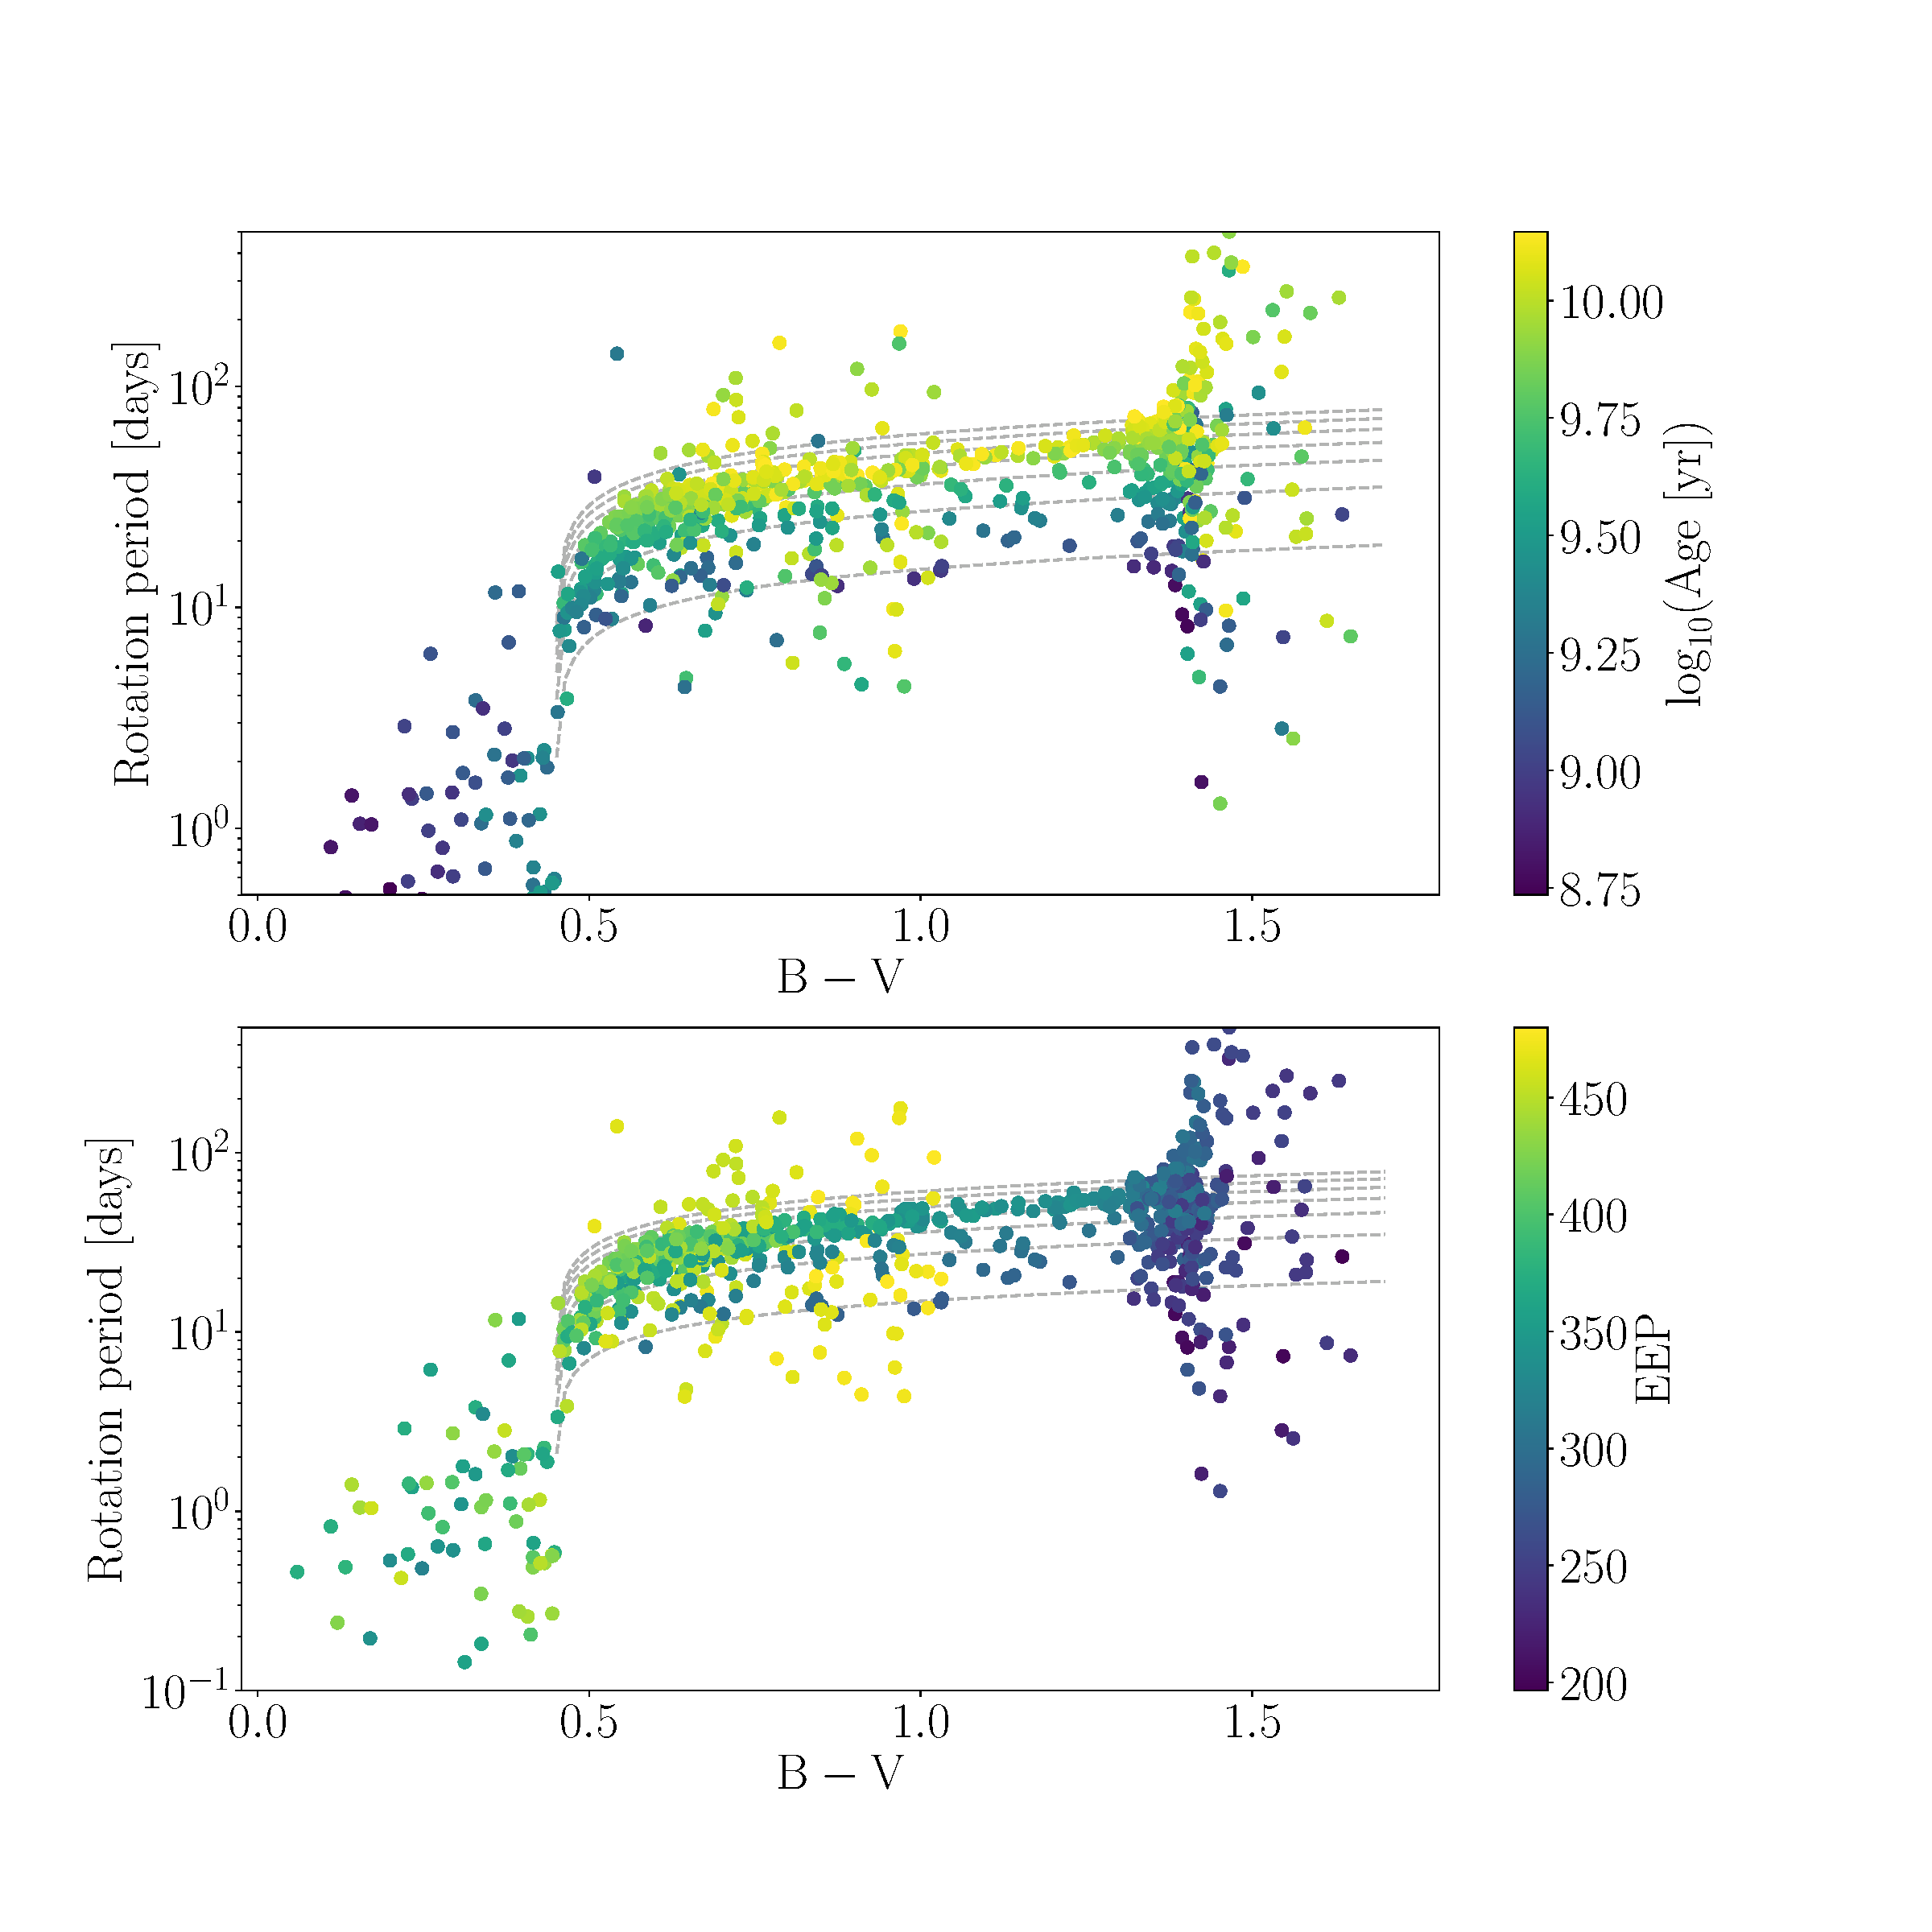
\includegraphics[width=1.\textwidth]{rotation_model}
\label{fig:rotation_model}
\end{figure}

The rotation periods of hot stars, cool stars, subgiants and giants evolve
differently to FGK and early M dwarfs.
Stars more massive than around 1.25 M$_\odot$, with a temperature $\gtrsim$
6250 K and a $B-V$ color $\lesssim$ 0.45 do not spin down appreciably over
their main sequence lifetimes since they do not have the deep convective
envelope needed to generate strong magnetic fields.
Late M dwarfs with masses $\lesssim$ 0.3 M$_\odot$, temperatures $\lesssim$
3500 and $B-V$ $\gtrsim$ 1.4 do not start magnetic braking until at least
after the age of Praesepe ($\sim$650 million years).
Both hot and cool stars retain rotation periods that are similar to their
primordial distribution \citep[see \eg][]{matt2012}.
Finally, the rotation periods of evolved stars slow dramatically as their
radii grow.
The empirical gyrochronology relation described above does not include these
stars, however it is still possible to infer the ages of hot and evolved stars
using isochrone fitting (unfortunately neither gyrochronology nor isochrone
fitting works well for late M dwarfs).
In order to `switch off' gyrochronology, and just use isochrone fitting for
the hot, cool and evolved stars, we designed a model describing the rotation
period variance of these stars, inflating the variance to high values in
regions of parameter space where gyrochronology does not apply.
The variance model was designed to reflect the observed distributions of hot,
cool and evolved stars, however its main purpose is to artificially reduce the
amount of age-information carried by rotation periods for stars where the
rotation period is uninformative.
We used three sigmoid functions to increase the standard deviation of the
rotation period distributions of hot, cool and evolved stars which are shown
in figure \ref{fig:variance}.
This additional variance is zero where gyrochronology works well: FGK and
early M dwarfs and 0.25 ($\sigma = 0.5$) for hot, cool and evolved stars.
The logistic functions shown in figure \ref{fig:variance} reach half their
maximum values at 0.45, 1.4 and 454 for hot stars, cool stars and subgiants,
respectively.
The maximum standard deviation value of all three groups (hot, cool and
evolved) is 0.5 and the logistic growth rate, or steepness, of the three
sigmoids are 100, 100 and .2 for hot, cool and evolved stars respectively.
If a star is both hot and evolved, the additional standard deviation of its
rotation period will rise to 1 (no late M dwarfs have yet evolved off the main
sequence so this will not apply to the cool stars).
The (log) rotation periods of hot stars are modelled as a broad Gaussian with
a mean of 0 (1 day in linear rotation period) and a standard deviation of
0.5.
The (log) rotation periods of cool and evolved stars were modelled as a
Gaussian with mean given by the log of equation \ref{eqn:gyro} and standard
deviations of 0.5.
\begin{figure}
  \caption{
    The additional standard deviation in rotation period added to the
    observational period uncertainties in our model.
    The standard deviation was artificially increased for early F stars ($B-V
    < 0.45$), late M dwarfs ($B-V > 1.4$) and evolved stars (EEP $>$ 454) in
    order to down-weight the age-information supplied by rotation periods.
    The rotation periods of these stars do not follow the deterministic
    gyrochronology relation and their ages should mostly be inferred via
    isochrone fitting.
    Down-weighting the gyrochronal likelihood by the inverse variance
    ($1/\sigma^2$) allows the ages of these stars to be mostly inferred
    via isochrone fitting.
    The ages of hot and evolved stars can be relatively precisely constrained
    with isochrone fitting since their position on the CMD changes
    rapidly with time, however isochrone fitting cannot constrain the ages of
    late M dwarfs, so the age of any star with $B-V > 1.4$ will not be
    precisely constrained with \sd.
}
  \centering
    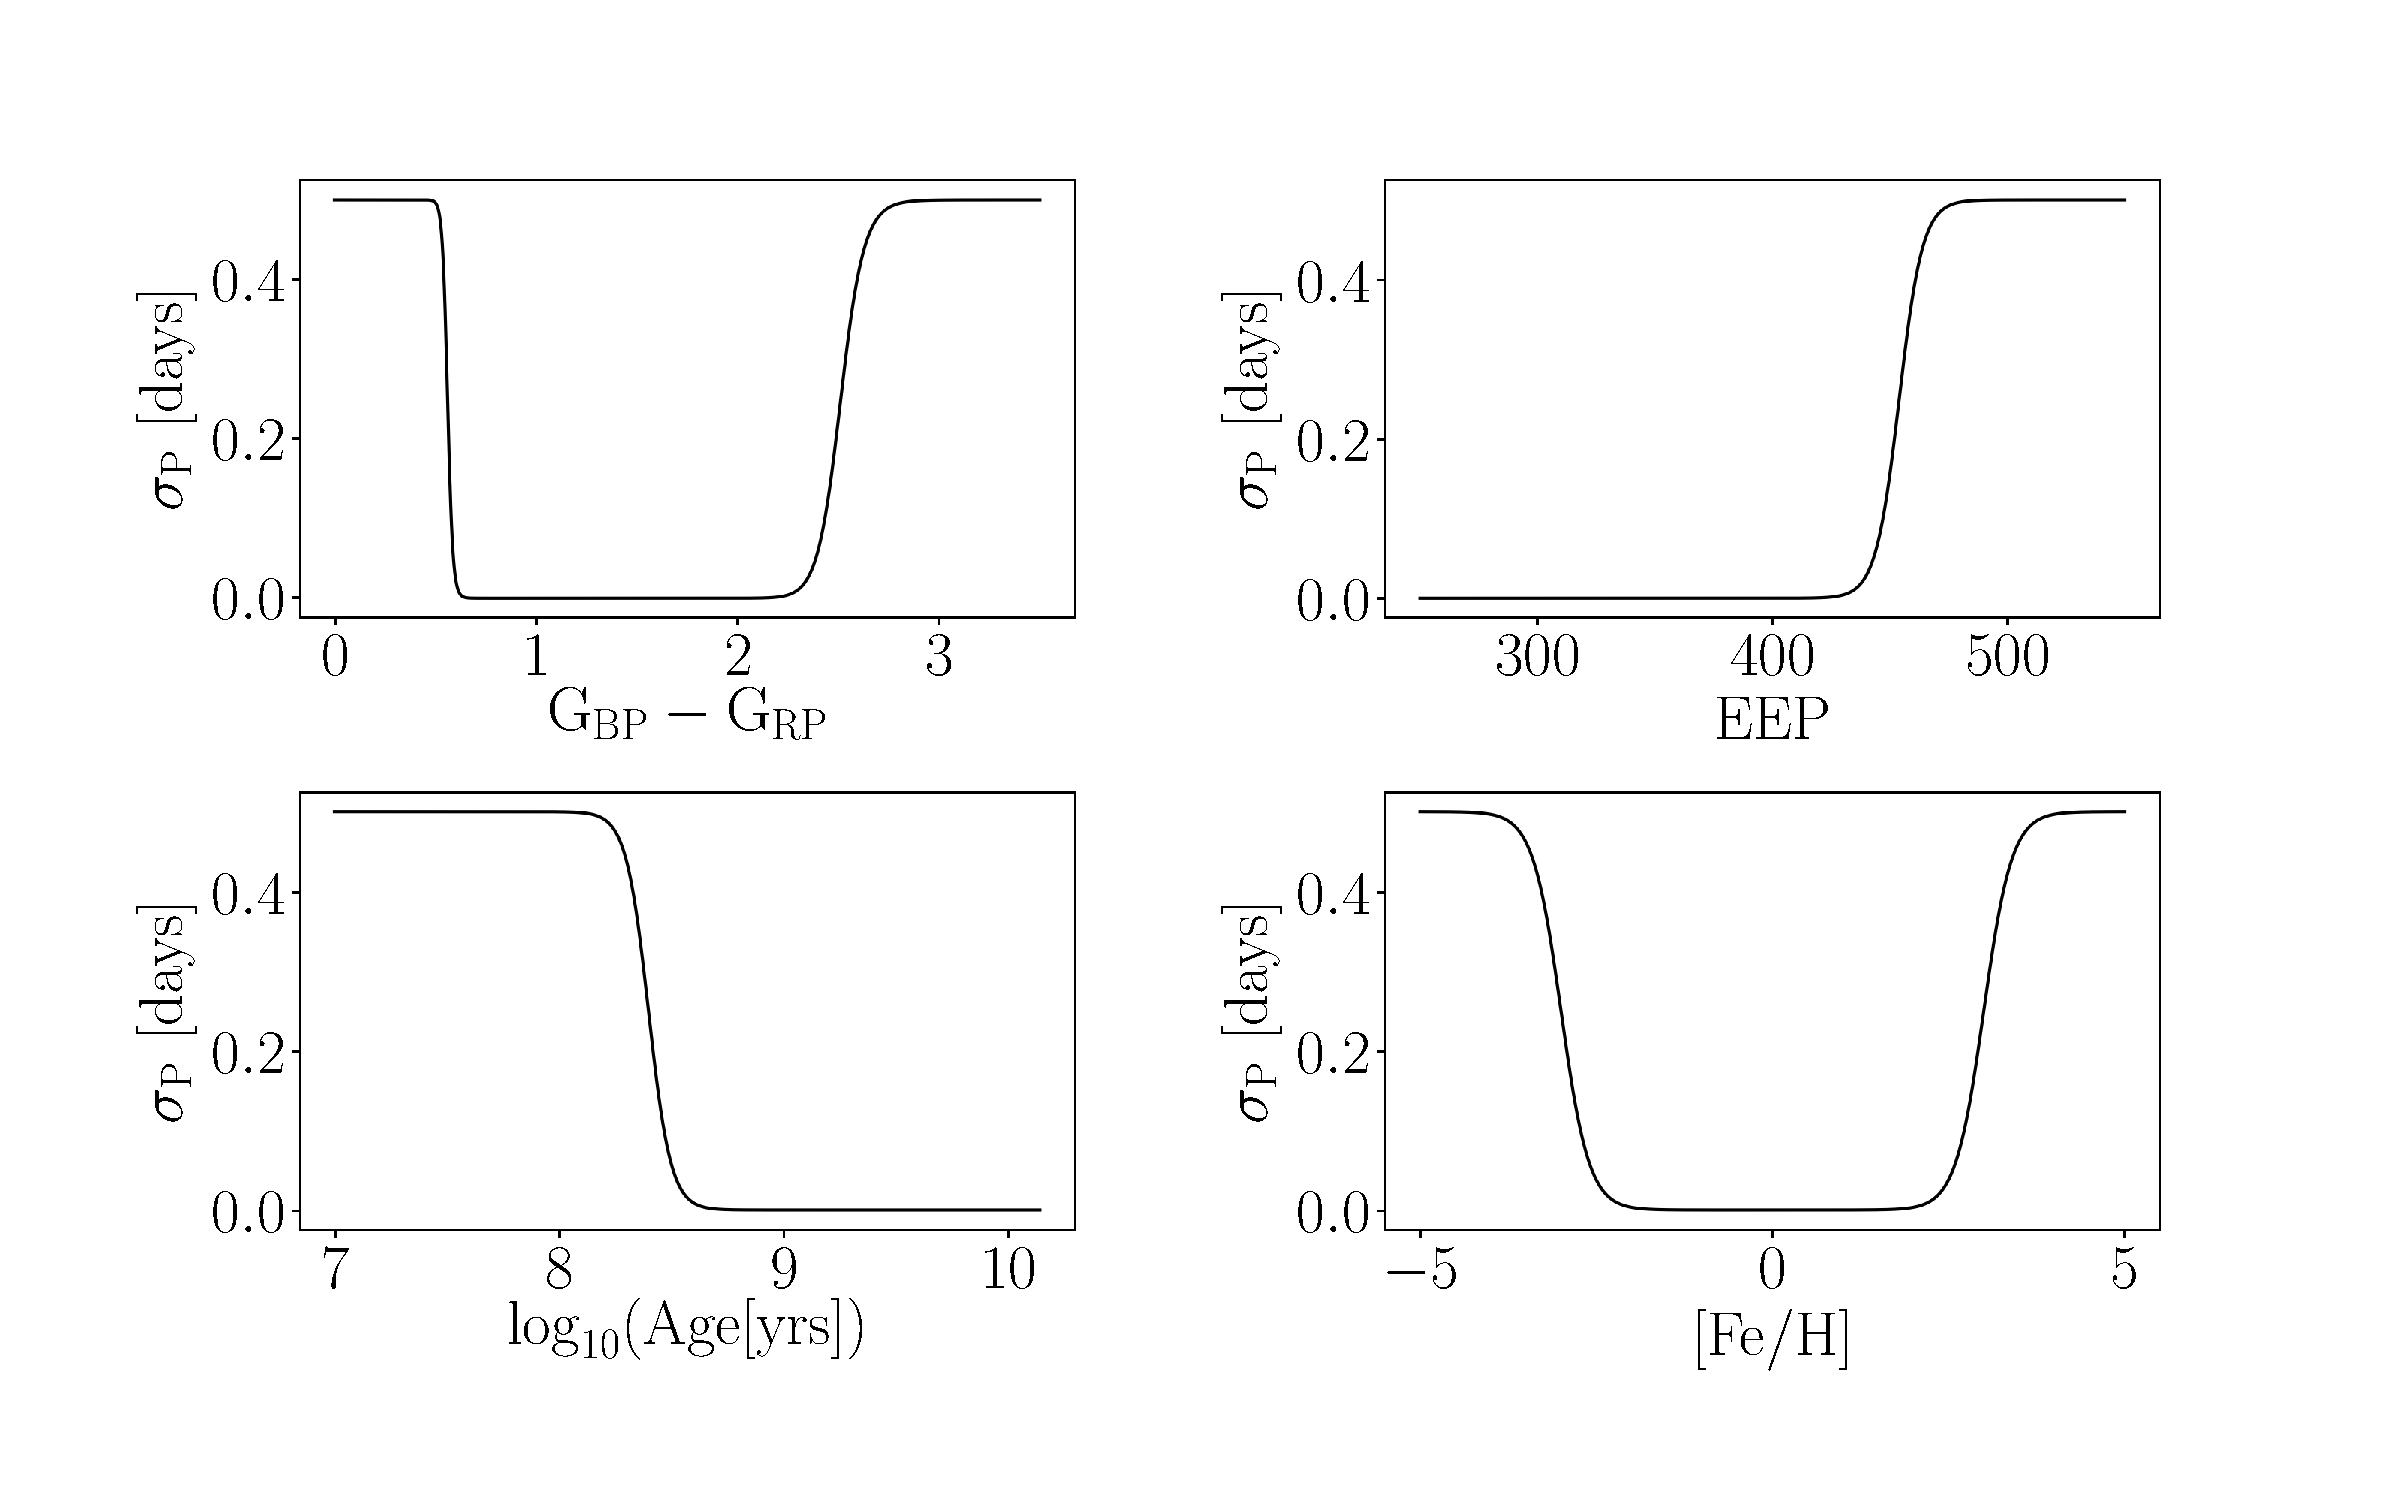
\includegraphics[width=1.\textwidth]{variance}
\label{fig:variance}
\end{figure}


% The rotation periods of evolved stars (EEP $>454$ were modelled with equation
% \ref{eqn:gyro}, however the uncertainties were artificially increased, by 10
% days, to account for the large amount of scatter expected in the rotation
% periods of these stars.
% The resulting rotation period model for evolved stars is a stochastic version
% of the above equation for MS stars where rotation periods are drawn from a
% broad Gaussian with equation \ref{eqn:gyro} as the mean function and the
% (rotation period uncertainty + 10)$^2$ as the variance.
% The number ten was chosen somewhat arbitrarily but we found that the resulting
% age estimates were relatively insensitive to this choice as long as the
% rotation periods were uncertain enough to allow isochrone fitting to dominate
% the age information.
% Hot stars ($B-V < 0.45$) and late M dwarfs ($B-V \gsim 1.25$) were treated
% differently again.
% Hot stars retain their primordial rapid rotation periods since they do not
% have the deep convective envelope needed to generate strong magnetic fields.
% Very cool stars have not yet begun to spin down and also retain
% rotation periods that is similar to their primordial distribution \citep[see
% \eg][]{matt2012}.
% The rotation periods of these stars were modeled with a Gaussian in log-space,
% with parameters based on the distribution of M dwarf rotation periods in the
% Praesepe cluster: a mean of 0.5 and variance of 0.55,
% \begin{equation}
%     \log_{10}(P_\mathrm{rot})\sim\mathcal{N}(0.5, 0.55).
% \end{equation}

% Because this gyochronology model is not calibrated to include stars turning
% off the main sequence whose rotation slows rapidly due to their increasing
% radius, we do not apply gyrochronology to stars with a MIST model \eep\
% greater than 454 as this corresponds to terminal age \ms\ \citep{dotter2016,
% choi2016}.
% In future, rather than switch gyrochronology off at a certain \eep, we could
% include it as an additional dimension and model rotation periods as a function
% of it.
% \footnote{This number was determined by investigating the
% correspondance between \eep\ and position on the HR diagram.
% See the {\it Jupyter} notebook at
% \url{https://github.com/RuthAngus/stardate/blob/master/paper/code/EEP_cutoff.ipynb}.
% In future, \eep\ could be used as a parameter in our gyrochronology model.
% }.
% In addition, stars with \cbv $>$ 0.45, corresponding to a temperature around
% 6250 K  only modeled using isochrones, not gyrochronology.
% These stars have thin convective envelopes and do not spin down substantially
% over their \ms\ lifetimes so their rotation periods do not strongly predict
% their ages.
% However, isochrone fitting can provide relatively precise ages for these hot
% stars, as well as evolved stars with large \eep s.

% It was recently shown that a simple power law in age does not provide a good
% fit to old asteroseismic stars \citep{angus2015, vansaders2016}.
% It is hypothesized that the magnetic braking of these old stars has ceased and
% cannot be modeled with a Skumanich-like spin-down law \citep{vansaders2016}.
% In future, the above model could and should be updated to include a more
% flexible treatment of rotation period as a function of age in order to account
% for the change of slope in the relation.
% Until then, this method should only be used for stars with Rossby number below
% 2.1 \citep{vansaders2016}, \ie\ their ratio of rotation period to convection
% overturn time ($P/\tau = Ro$) does not exceed 2.1.
% In this work we are chiefly concerned with introducing a new framework where
% rotation periods are modeled {\it simultaneously} with isochronal features.
% Although the gyrochronology models used here do not provide a good fit to all
% the available data, we reiterate that no single model {\it is} able to
% reproduce all the data, and that there is utility in using such a simple,
% linear, empirical model like this.
% Again, we are not attempting to improve gyrochronology models in this work:
% in this paper we are more concerned with introducing a new approach to
% modeling
% This method is highly flexible and modular and an improved gyrochronology
% model could easily be swapped in for this one in future.
% For example, a linear combination of {\it physical} parameters such as \logg,
% \feh, and mass or \teff\ could be to be used to predict an age from a rotation
% period.

%   - Emcee, including assessing convergence.
When applying our model to infer the age of a star, we sampled the joint
posterior PDF over age, mass, metallicity, distance and extinction using the
affine invariant ensemble sampler, {\tt emcee} \citep{foreman-mackey2013} with
24 walkers.
Samples were drawn from the posterior PDF until 100 {\it independent} samples
were obtained.
We actively estimated the autocorrelation length, which indicates how many
steps were taken per independent sample, after every 100 steps using the
autocorrelation tool built into {\tt emcee}.
The MCMC concluded when {\it either} 100 times the autocorrelation length was
reached and the change in autocorrelation length over 100 samples was less
than 0.01, {\it or} the maximum of 100,000 samples was obtained.
This method is trivially parallelizable, since the inference process for each
star can be performed on a separate core.
The age of a single star can be inferred in around 10 minutes on a laptop
computer.

% Although the gyrochronology model described above \citep[equation
% \ref{eqn:gyro},][]{angus2015} has been calibrated using a number of cluster
% stars, it does not provide a good fit to any individual cluster.
% No current gyrochronology model is able to capture the behavior of rotation as
% a function of color and age for individual benchmark clusters: the shape of
% this relation is different in each and current models are not flexible enough
% to capture inter-cluster differences in rotational evolution.
% For this reason, we also explored the rotational evolution of a single
% cluster, in order to produce a best-case model and demonstrate the potential
% of rotation-dating in a case where the model is perfectly accurate.
% We chose Praesepe as it is a relatively old open cluster \citep[$\sim$ 600
% Myrs][]{gossage2018}, meaning its Solar-type members have converged onto the
% rotational main sequence, and it is relatively compact on the sky so many of
% its members were observed during a single \ktwo\ campaign.
% In fact, Praesepe was repeatedly observed by \ktwo, in Campaigns 5, 16 and 18,
% however we only use rotation periods published from the analysis of Campaign 5
% in this work \citep{rebull2016}.

% % The Praesepe model
% We used a three-dimensional polynomial model to predict rotation period as a
% function of \gaia\ color and age for Praesepe and the Sun.
% This model consists of a 4th order polynomial in logarithmic Gaia color:
% $G_{Bp} - G_{Rp}$, which we write as $C_G$ for simplicity, and a 1st order
% polynomial (a straight line) in logarithmic age.
% We used \gcolor\ instead of (B-V) because, due to the $\sim$ billion stars
% observed by \gaia, it is now the most abundant and widely available
% photometric color.
% Our gyrochronology likelihood function is designed to compare observed
% rotation period to predicted rotation period.
% For this reason the gyrochronology model we used must predict rotation period
% as a function of age and color.
% However, when {\it calibrating} the gyrochronology model, we chose to make
% {\it age} the dependent variable because the uncertainties on age are much
% greater than the uncertainties on rotation period.
% Since we are using a linear model, the relation is easily invertable.
% We fitted the following model to Praesepe members:
% \begin{equation}
%     \log_{10}(A) = a + b\log_{10}(C_G) + c\log_{10}^2(C_G) +
%     d\log_{10}^3(C_G) + e\log_{10}^4(C_G) + f\log_{10}(P)
% \label{eqn:gyro_age_praesepe}
% \end{equation}
% where $P$ is rotation period in days, $C_G$ is Gaia color, $A$ is stellar age
% in years and the lower case letters are free parameters which we fitted to the
% data using linear least squares.
% We adopted an age for Praesepe of 600 million years \citep{gossage2018}, a
% Solar age of 4.56 Gyr \citep{connelly2012}, and a Solar rotation period of 26
% days \citep[][Morris \etal, in prep]{balthasar1986, howe2000}.
% The Sun's color in the Gaia color bandpasses, $G_{Bp} - G_{Rp}$, is 0.82
% \citep{casagrande2018}.
% We found best-fit values: $a = 7.37 \pm 0.03, b = -1.4 \pm 0.1, c = 5.0 \pm
% 0.8, d = -34 \pm 3, e = 66 \pm 14$, and $f = 1.49 \pm 0.02$.
% Rotation periods for Prasepe were obtained from \citet{rebull2017} and their
% \gaia\ colors were obtained by crossmatching their sky-projected positions
% with the \gaia\ DR2 catalog.
% % The $f$ parameter is the inverse of the slope of the rotation period and age
% % which was originally measured to be around 0.5.
% % Our Praesepe and Sun-only fit results in a slightly steeper age dependence of
% % around 0.67, however this value is likely be
% We inverted this relation to predict rotation period as a function of color
% and age,
% \begin{equation}
%     \log_{10}(P) = \frac{\log_{10}(A) - a - b\log_{10}(C_G) - c\log_{10}^2(C_G) -
%     d\log_{10}^3(C_G) - e\log_{10}^4(C_G)}{f}.
% \label{eqn:gyro_age_praesepe}
% \end{equation}
% Both gyrochronology models of equations \ref{eqn:gyro} and
% \ref{eqn:gyro_age_praesepe} are used to predict the ages of individual
% Praesepe stars from their rotation periods and apparent magnitudes in section
% \ref{section:results}.

% % The PGM
% \begin{figure}
%   \caption{
% A probabilistic graphical model (PGM) showing the conditional
% dependencies between the parameters (white nodes) and
% observables (gray nodes) in our model.
% % ${\bf \theta}$ is a vector of {\it parameters}: mass, observed bulk
% %     metallicity, distance and V-band extinction; and ${\bf O}$ is a vector of
% %     {\it observables}: apparent magnitudes, $m_x$, effective temperature,
% %     \teff, surface gravity, \logg, observed bulk metallicity, $\hat{F}$, and
% %     parallax, $\bar{\omega}$.
% % determined by the mass, $M$, age, $A$, distance, $D$, extinction, $A_V$
% % and bulk metallicity, $F$, of a star.
% ${\bf \theta}$ is a vector of {\it parameters}: mass, observed bulk
%     metallicity, distance and V-band extinction; and ${\bf O}$ is a vector of
%     {\it observables}: apparent magnitudes, effective temperature, surface
%     gravity, observed bulk metallicity, and parallax.
%     The observables, ${\bf O}$, are determined by the parameters, $A$ and
%     ${\bf \theta}$.
%     $C_{B-V}$ is a latent parameter that is also determined by the parameters
%     $A$ and ${\bf \theta}$.
%     In our model, the rotation period observable, $P$, is determined {\it
%     only} by the age, $A$, and color ${C_{B-V}}$ parameters.
% The dependencies of observables on parameters and parameters on parameters are
%     indicated by arrows that start at a `parent' node and end at the dependent
%     observable, or `child' node.
% In our model, rotation period does not directly depend on distance,
% extinction, metallicity or mass, only age and B-V color.
% This PGM is a representation of the factorized joint PDF over parameters and
% observables of equation \ref{eqn:factorized}.
% }
%   \centering
%     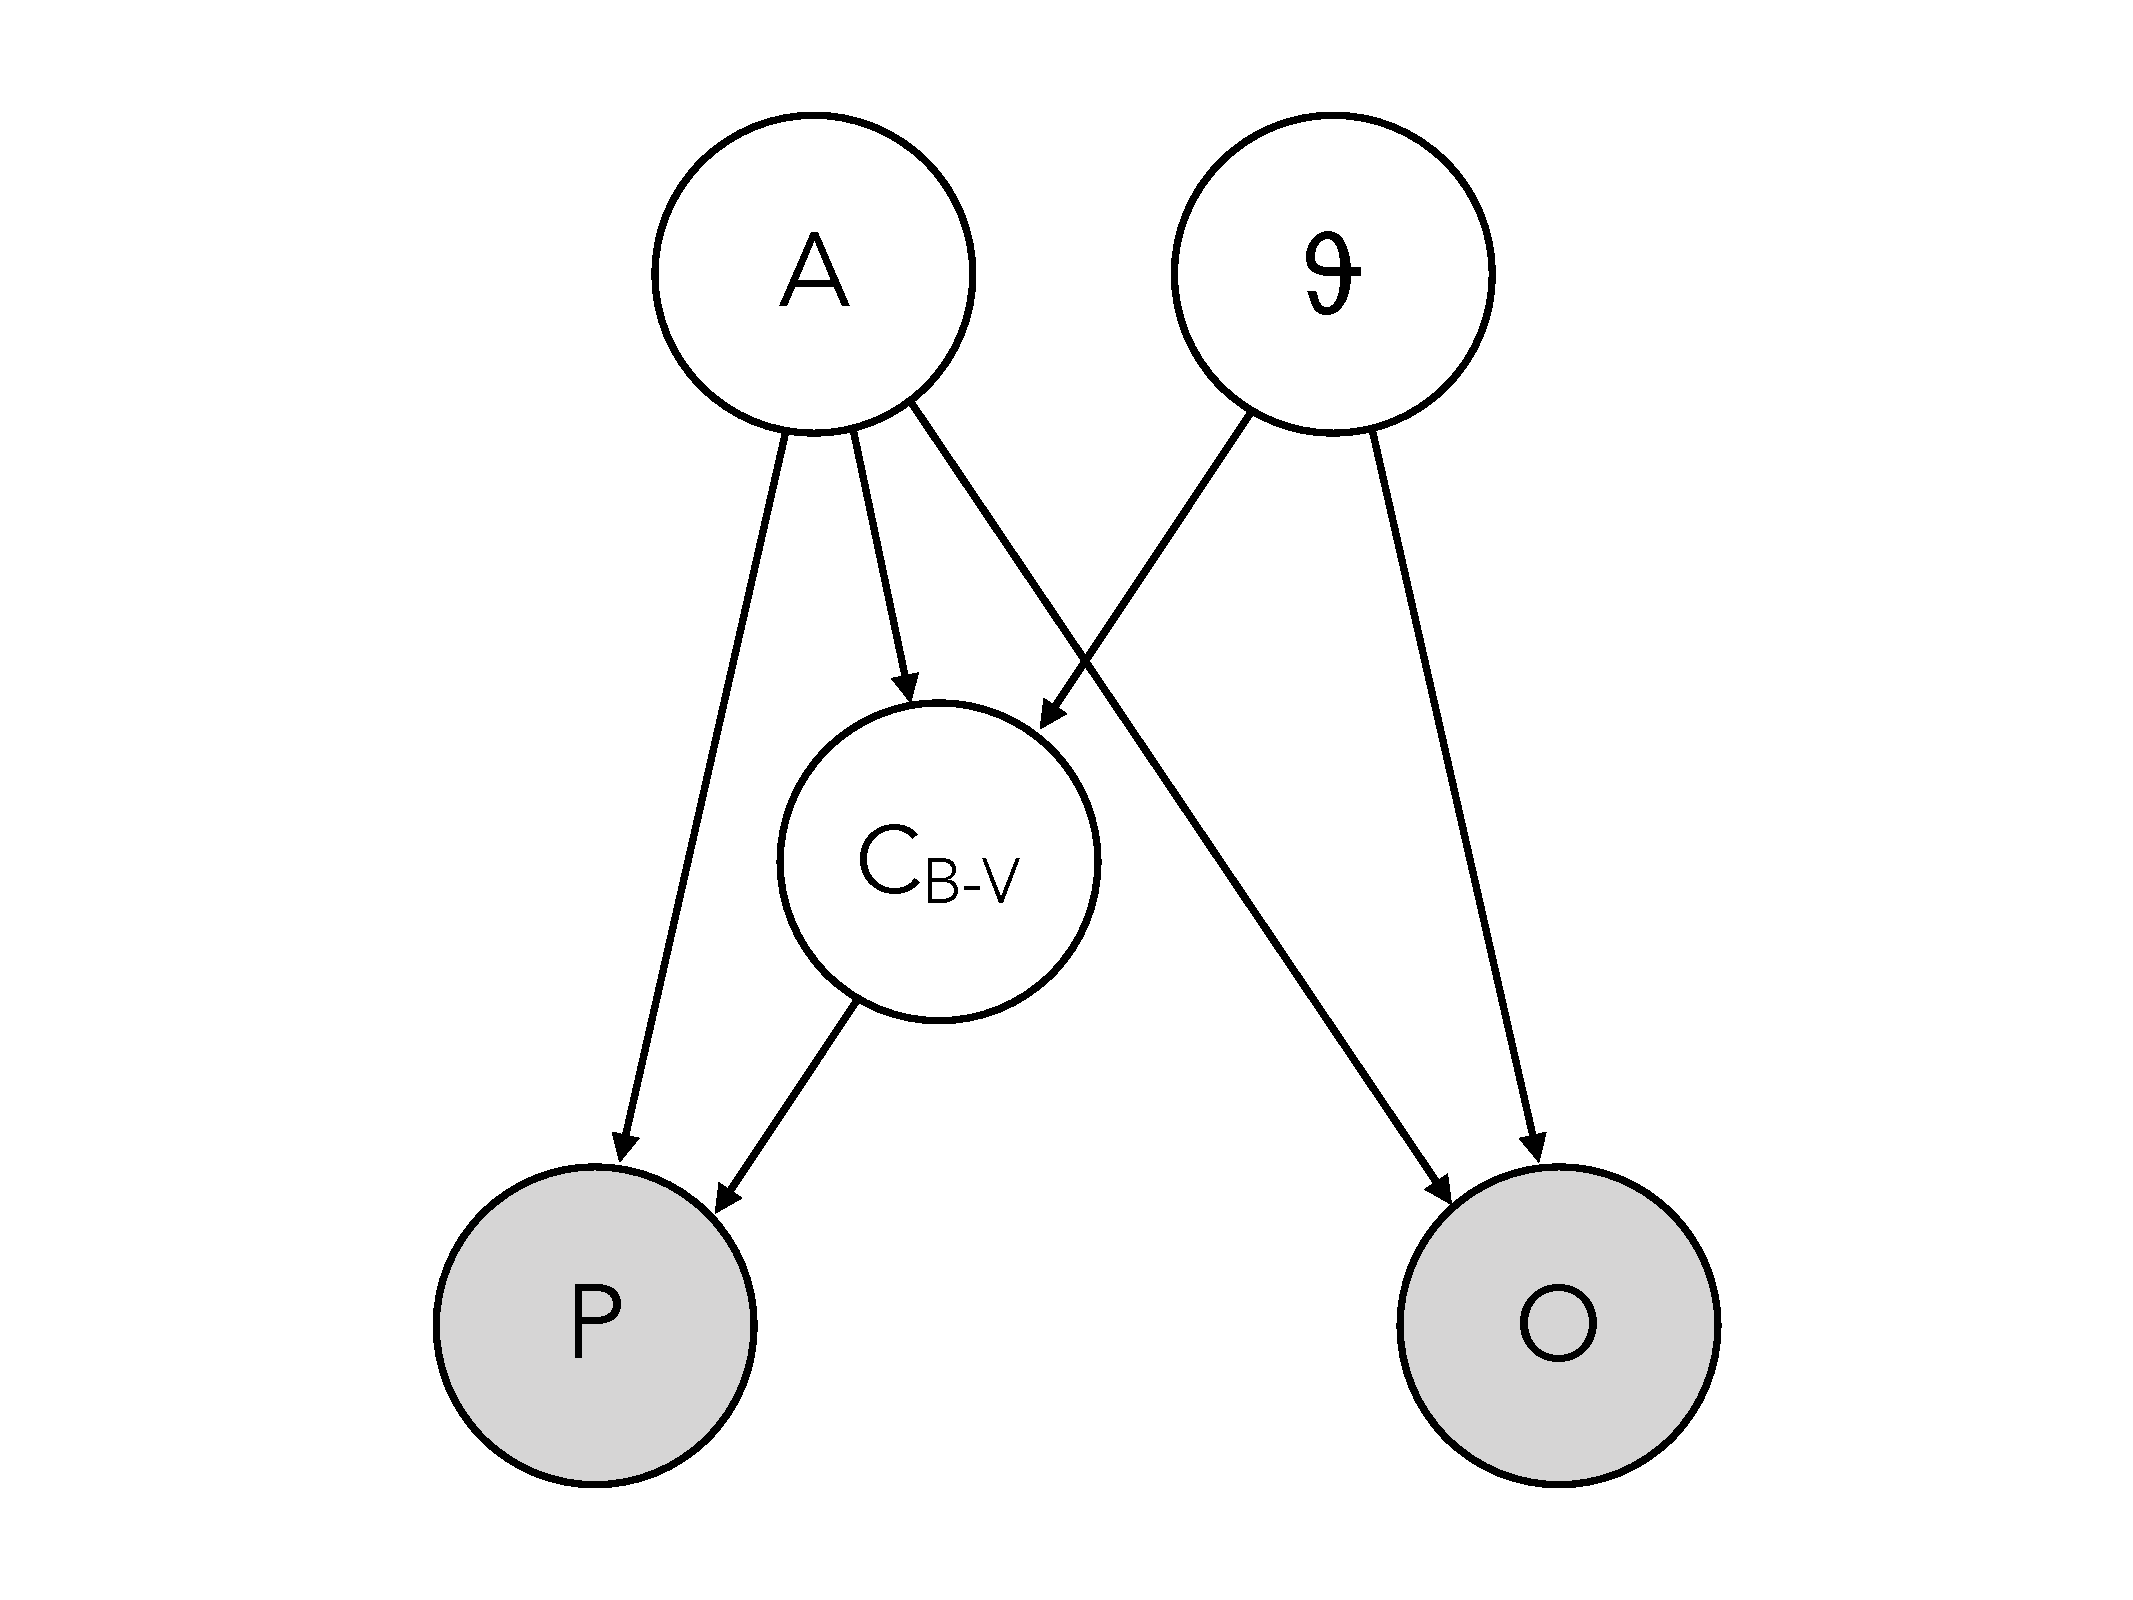
\includegraphics[width=.7\textwidth]{PGM}
% \label{fig:PGM}
% \end{figure}
